\section{结果：单体序列恢复与甲基化分类}
\label{sec:results-monomer}

\subsection{Ser 来源修正改变评价真值，但不改变模型输出}

单体留出集包含151条肽、1505个真实残基位点。来源复核后，旧标签中62个被写为 N-甲基 Ser 的位点改回天然 Ser；因此，论文主评价集由261个甲基化阳性和1244个阴性组成，阳性率为 $261/1505=17.34\%$。这一修正没有改变原始 \path{frankenstein_v28.pt} 的权重、基础氨基酸预测、甲基化概率或样本划分，改变的只有用于计算二分类指标的真值标签。

为避免把旧323阳性标签与修正真值混用，\path{data/Monomer_Corrected_1505.csv} 已将严格天然化输入的冻结概率逐位连接到修正 JSONL，并显式保留旧标签、修正标签、62个修正标志和阈值 $>0.6$ 的判定列；三种输入模式的原始4515行推理表另存为 \path{data/Monomer_RawPredictions_4515.csv}，只作来源追溯。

所有正文结果均排除 padding，并使用严格判定 $p>0.6$。旧标签及把 padding 计入分母的终端截图不参与正文估计；其来源和批大小依赖性仅在附录历史审计中说明（见\cref{app:historical}）。

\subsection{两个 Rosetta 来源面板的描述性分层}

测试集的 83 条 \path{Me_} 记录来自 Rosetta-2023 面板，68 条 \path{pdb_} 记录来自 Rosetta-2025 面板；两者都不是 Baker 实验结构。分层结果见\cref{tab:monomer-source-strata}。Rosetta-2025 面板的 RAA 和 F1 较高，但两个面板在构建版本、序列组成、长度和甲基阳性率上均可能不同，故这些差异只作异质性描述，不能解释为 Rosetta 版本升级或模型在某来源上的因果增益。

\begin{table}[H]
  \centering
  \caption{Ser 来源修正后，单体测试集按 Rosetta 理论结构面板分层的结果。F1 均使用严格 $p>0.6$。}
  \label{tab:monomer-source-strata}
  \begin{tabular}{L{35mm}C{30mm}C{19mm}C{31mm}C{31mm}}
    \toprule
    来源面板 & 单体/位点/阳性 & RAA & 已知序列 AUC/F1 & 端到端 AUC/F1 \\
    \midrule
    Rosetta-2023（\path{Me_}） & 83/763/114 & 12.19\% & 0.920/45.83\% & 0.931/51.90\% \\
    Rosetta-2025（\path{pdb_}） & 68/742/147 & 20.08\% & 0.886/59.69\% & 0.890/61.40\% \\
    \bottomrule
  \end{tabular}
\end{table}

\subsection{RAA 与联合扩展 token 恢复率}

天然化后，基础氨基酸预测正确242个位点，故单体 RAA 为
\begin{equation}
  \mathrm{RAA}=\frac{242}{1505}=16.08\%.
\end{equation}
RAA 只检验天然氨基酸类别，不评价甲基化状态。进一步要求“天然氨基酸类别正确，且在严格 $p>0.6$ 下甲基化状态也正确”时，224个位点满足条件，联合扩展 token 恢复率为
\begin{equation}
  \mathrm{Joint\ token\ recovery}=\frac{224}{1505}=14.88\%.
\end{equation}
端到端甲基二分类共有111个 TP，但其中只有20个位点的天然氨基酸类别也预测正确，另外91个位点虽然被判为甲基化，却甲基化了错误的氨基酸。因此，真实甲基残基的身份完全恢复率只有
\begin{equation}
  \mathrm{Exact\ methylated\mbox{-}residue\ recovery}=\frac{20}{261}=7.66\%.
\end{equation}
非甲基位点中另有204个位点同时预测对天然氨基酸和非甲基状态，故联合扩展 token 恢复为 $(20+204)/1505=224/1505$。天然化 RAA 的242个正确位点还包括17个“氨基酸正确但甲基漏检”和1个“氨基酸正确但误报甲基”的位置，所以 RAA 与联合 token 恢复相差18个位点。

\begin{table}[H]
  \centering
  \begin{threeparttable}
    \caption{原始 V28 在 Ser 来源修正单体留出集上的序列级结果。}
    \label{tab:monomer-sequence-recovery}
    \begin{tabular}{L{48mm}C{22mm}C{22mm}L{48mm}}
      \toprule
      指标 & 计数 & 比例 & 含义 \\
      \midrule
      天然化氨基酸恢复率（RAA） & $242/1505$ & 16.08\% & 只要求天然氨基酸类别正确 \\
      联合扩展 token 恢复率 & $224/1505$ & 14.88\% & 同时要求天然氨基酸类别和甲基化状态正确 \\
      端到端真实甲基残基身份完全恢复 & $20/261$ & 7.66\% & 只在真实甲基位点中，同时要求氨基酸身份与甲基状态正确 \\
      RAA 正确但甲基状态错误 & $18/1505$ & 1.20\% & 不能计作完整扩展 token 恢复 \\
      \bottomrule
    \end{tabular}
    \begin{tablenotes}[flushleft]\footnotesize
      \item 注：甲基化状态采用严格 $p>0.6$；分母仅含1505个真实残基，不含 padding。
    \end{tablenotes}
  \end{threeparttable}
\end{table}

\subsection{已知天然序列与端到端甲基化分类}

在已知天然序列条件下，模型直接按真实天然残基类别选择甲基化专家头；在端到端条件下，则先预测天然残基，再按预测类别选择专家头。因此，前者衡量甲基化头本身，后者还包含基础序列错误的级联影响。

已知天然序列任务的 ROC-AUC 为0.9003。在严格 $p>0.6$ 时，混淆矩阵为 $TP=121$、$TN=1176$、$FP=68$、$FN=140$；Accuracy、Precision、Recall、F1 和假阳性率分别为86.18\%、64.02\%、46.36\%、53.78\% 和5.47\%。模型在该口径下预测189个阳性位点，预测阳性率为12.56\%，低于修正真值的17.34\%。

端到端任务的 ROC-AUC 为0.9082。在同一严格阈值下，$TP=111$、$TN=1230$、$FP=14$、$FN=150$。对应 Accuracy 与 Precision 为89.10\%和88.80\%，Recall 与 F1 为42.53\%和57.51\%，假阳性率为1.13\%。端到端路径只预测125个阳性位点，预测阳性率为8.31\%。相较已知天然序列任务，它减少了54个假阳性，但同时少识别10个真阳性；因此，较高的 Accuracy、Precision 或 AUC 不能解释为所有方面均优于已知序列任务。

\begin{table}[H]
  \centering
  \caption{Ser 来源修正标签下的单体甲基化分类结果（严格 $p>0.6$）。}
  \label{tab:monomer-methyl-classification}
  \resizebox{\textwidth}{!}{%
    \begin{tabular}{lrrrrrrrrrrr}
      \toprule
      任务 & AUC & TP & TN & FP & FN & Accuracy & Precision & Recall & F1 & FPR & 预测阳性率 \\
      \midrule
      已知天然序列 & 0.9003 & 121 & 1176 & 68 & 140 & 86.18\% & 64.02\% & 46.36\% & 53.78\% & 5.47\% & 12.56\% \\
      端到端 & 0.9082 & 111 & 1230 & 14 & 150 & 89.10\% & 88.80\% & 42.53\% & 57.51\% & 1.13\% & 8.31\% \\
      \bottomrule
    \end{tabular}%
  }
  \begin{minipage}{\textwidth}
    \footnotesize 注：两项任务共享261个阳性和1244个阴性真值。AUC 为阈值无关的排序指标；其余指标均在预设严格阈值 $p>0.6$ 下计算。
  \end{minipage}
\end{table}

\begin{figure}[H]
  \centering
  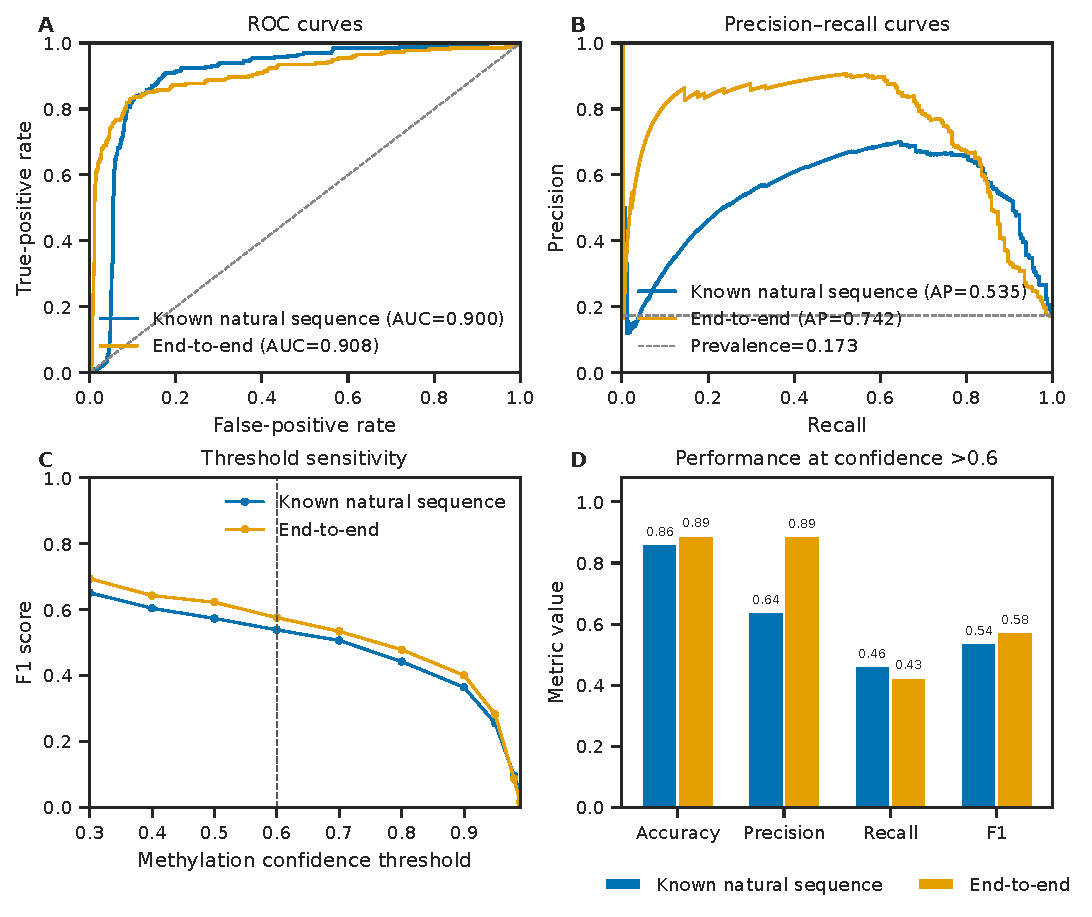
\includegraphics[width=0.98\textwidth]{figures/Fig4_original_checkpoint_model_performance.pdf}
  \caption{原始检查点在 Ser 来源修正单体留出集上的甲基化预测表现。A，ROC 曲线；B，精确率--召回率曲线；C，不同置信度阈值下的 F1；D，严格 $p>0.6$ 时的 Accuracy、Precision、Recall 与 F1。蓝色表示已知天然序列任务，橙色表示端到端任务。所有曲线和计数均来自1505个真实残基位点，不含 padding。}
  \label{fig:monomer-model-performance}
\end{figure}

\subsection{阈值结果的解释边界}

修正标签后，已知天然序列任务在阈值0.3处的 F1 高于阈值0.6，但0.3并非本文预设的部署阈值，而且该最大值是在同一留出集上观察得到。为避免用测试集反向挑选阈值，正文只报告预先冻结的严格 $p>0.6$ 结果，完整阈值敏感性由\cref{fig:monomer-model-performance}展示。若 RMC 表示端到端甲基阳性的二分类恢复，它等于 Recall，即 $111/261=42.53\%$；若要求真实甲基残基的天然氨基酸身份也正确，则为 $20/261=7.66\%$；若以全部位点为分母计算完整扩展 token 恢复，则为 $224/1505=14.88\%$。三者回答不同问题，本文不把它们混称为一个 RMC。

甲基二分类 Accuracy 较高也不等于完整序列设计准确。修正集阴性位点占82.66\%，而端到端 RAA 仅为16.08\%；只有联合 token 恢复率同时反映基础类别和甲基状态。正文因此并列报告 RAA、甲基分类指标和联合 token 恢复率，而不使用旧终端输出中的“Total End-to-End Acc”替代其中任何一项。

\subsection{原始 V28 没有可报告的单体结构结果}

单体 JSONL 中的坐标是 Rosetta 理论输入骨架，不是端到端设计序列的预测结构。现有 runbook 曾规划 explicit-methyl 与 naturalized 的 HighFold 结构任务，另有使用旧阈值0.30的参考/设计清单；但与本文阈值0.60相符的预测结构、成对结果表、PyRosetta 能量和通透性原始文件均不在可核验资产中。因此，原始 V28 的单体 CA/backbone/all-atom RMSD、甲基化位点 RMSD、pLDDT/pTM/PAE、能量、结构多样性和通透性均没有论文级数值。ipTM、界面 pLDDT、BSR 与受体框架姿态 RMSD对单链单体本身也不适用。上述项目明确记为“未计算/不适用”，而不是0；best85 或历史 V12 结果不得移植到 V28 单体队列。
